% Figure 6. Where the time goes in a STAR answer. Labels: LABELS.md, Figure 6.
% Drawn as a timing-diagram bus. Segments are to scale: 20, 10, 60, 10 of 900pt.
\def\eeprepfigure{1}
\providecommand{\eepstyledir}{../style}% repo: ../style
\input{\eepstyledir/circuitikz-preamble.tex}
% Colours, fonts, and text styles for the Get hired figures.
% Input after style/circuitikz-preamble.tex (in the repo: ../../style/circuitikz-preamble.tex).
% Define \eepdark before this file for the dark build. Same names as the resume figures,
% plus the rest of the navy palette. Crimson (eepaccent) marks one thing per figure.
\setmainfont{Newsreader}[
  BoldFont={Newsreader Bold},
  ItalicFont={Newsreader Italic},
  BoldItalicFont={Newsreader Bold Italic},
]
\usetikzlibrary{arrows.meta,calc,decorations.pathreplacing}
\ifdefined\eepdark
  \definecolor{eepink}{HTML}{ECEEF2}
  \definecolor{eeptext}{HTML}{D0D4DB}
  \definecolor{eepinktwo}{HTML}{A6AFBF}
  \definecolor{eepmute}{HTML}{8F95A0}
  \definecolor{eepsilver}{HTML}{76808F}
  \definecolor{eeprule}{HTML}{3B4352}
  \definecolor{eepwash}{HTML}{17243A}
  \definecolor{eepsunken}{HTML}{101828}
  \definecolor{eepfill}{HTML}{131C2E}
  \definecolor{eeppaper}{HTML}{0D1524}
  \definecolor{eepaccent}{HTML}{E06A5F}
  \definecolor{eepaccentsoft}{HTML}{2A1A24}
\else
  \definecolor{eepink}{HTML}{16233A}
  \definecolor{eeptext}{HTML}{232A39}
  \definecolor{eepinktwo}{HTML}{424D63}
  \definecolor{eepmute}{HTML}{5E636C}
  \definecolor{eepsilver}{HTML}{838C9A}
  \definecolor{eeprule}{HTML}{C4C8CF}
  \definecolor{eepwash}{HTML}{E7ECF3}
  \definecolor{eepsunken}{HTML}{F3F4F6}
  \definecolor{eepfill}{HTML}{FFFFFF}
  \definecolor{eeppaper}{HTML}{FBFBFC}
  \definecolor{eepaccent}{HTML}{A3201D}
  \definecolor{eepaccentsoft}{HTML}{F8ECEA}
\fi
% Draw in y-down points so coordinates read like a mockup: [x=1pt, y=-1pt].
\tikzset{
  eeptitle/.style={anchor=base west, inner sep=0pt, text=eepink, font=\rmfamily\bfseries\fontsize{26}{31}\selectfont},
  eephead/.style={inner sep=0pt, text=eepink, font=\sffamily\bfseries\fontsize{14.5}{18}\selectfont},
  eepbody/.style={inner sep=0pt, text=eepinktwo, font=\sffamily\fontsize{13}{17}\selectfont},
  eepnote/.style={inner sep=0pt, text=eepmute, font=\sffamily\fontsize{12.5}{16}\selectfont},
  eepsrc/.style={anchor=north west, inner sep=0pt, align=left, text=eepmute, font=\sffamily\fontsize{11}{14.5}\selectfont},
  eepbox/.style={draw=eepink, fill=eepfill, rounded corners=4pt},
  eepfocus/.style={draw=eepaccent, fill=eepfill, rounded corners=4pt, line width=1.8pt},
  eeparrow/.style={-{Stealth[length=8pt,width=6pt]}},
  eepdash/.style={dash pattern=on 4pt off 4pt},
  eeplead/.style={draw=eepsilver, line width=0.9pt},
}
% A dot on a trace, like a schematic junction.
\newcommand{\eepdot}[2][eepink]{\fill[#1] #2 circle (3.6pt);}
% Short labels never hyphenate.
\hyphenpenalty=10000 \exhyphenpenalty=10000
% One space after a full stop, as on the site.
\frenchspacing

% #1 start x, #2 end x, #3 style
\newcommand{\seg}[3]{\draw[#3, line join=miter] (#1,160) -- ({#1+7},140) -- ({#2-7},140) -- (#2,160) -- ({#2-7},180) -- ({#1+7},180) -- cycle;}
\begin{document}
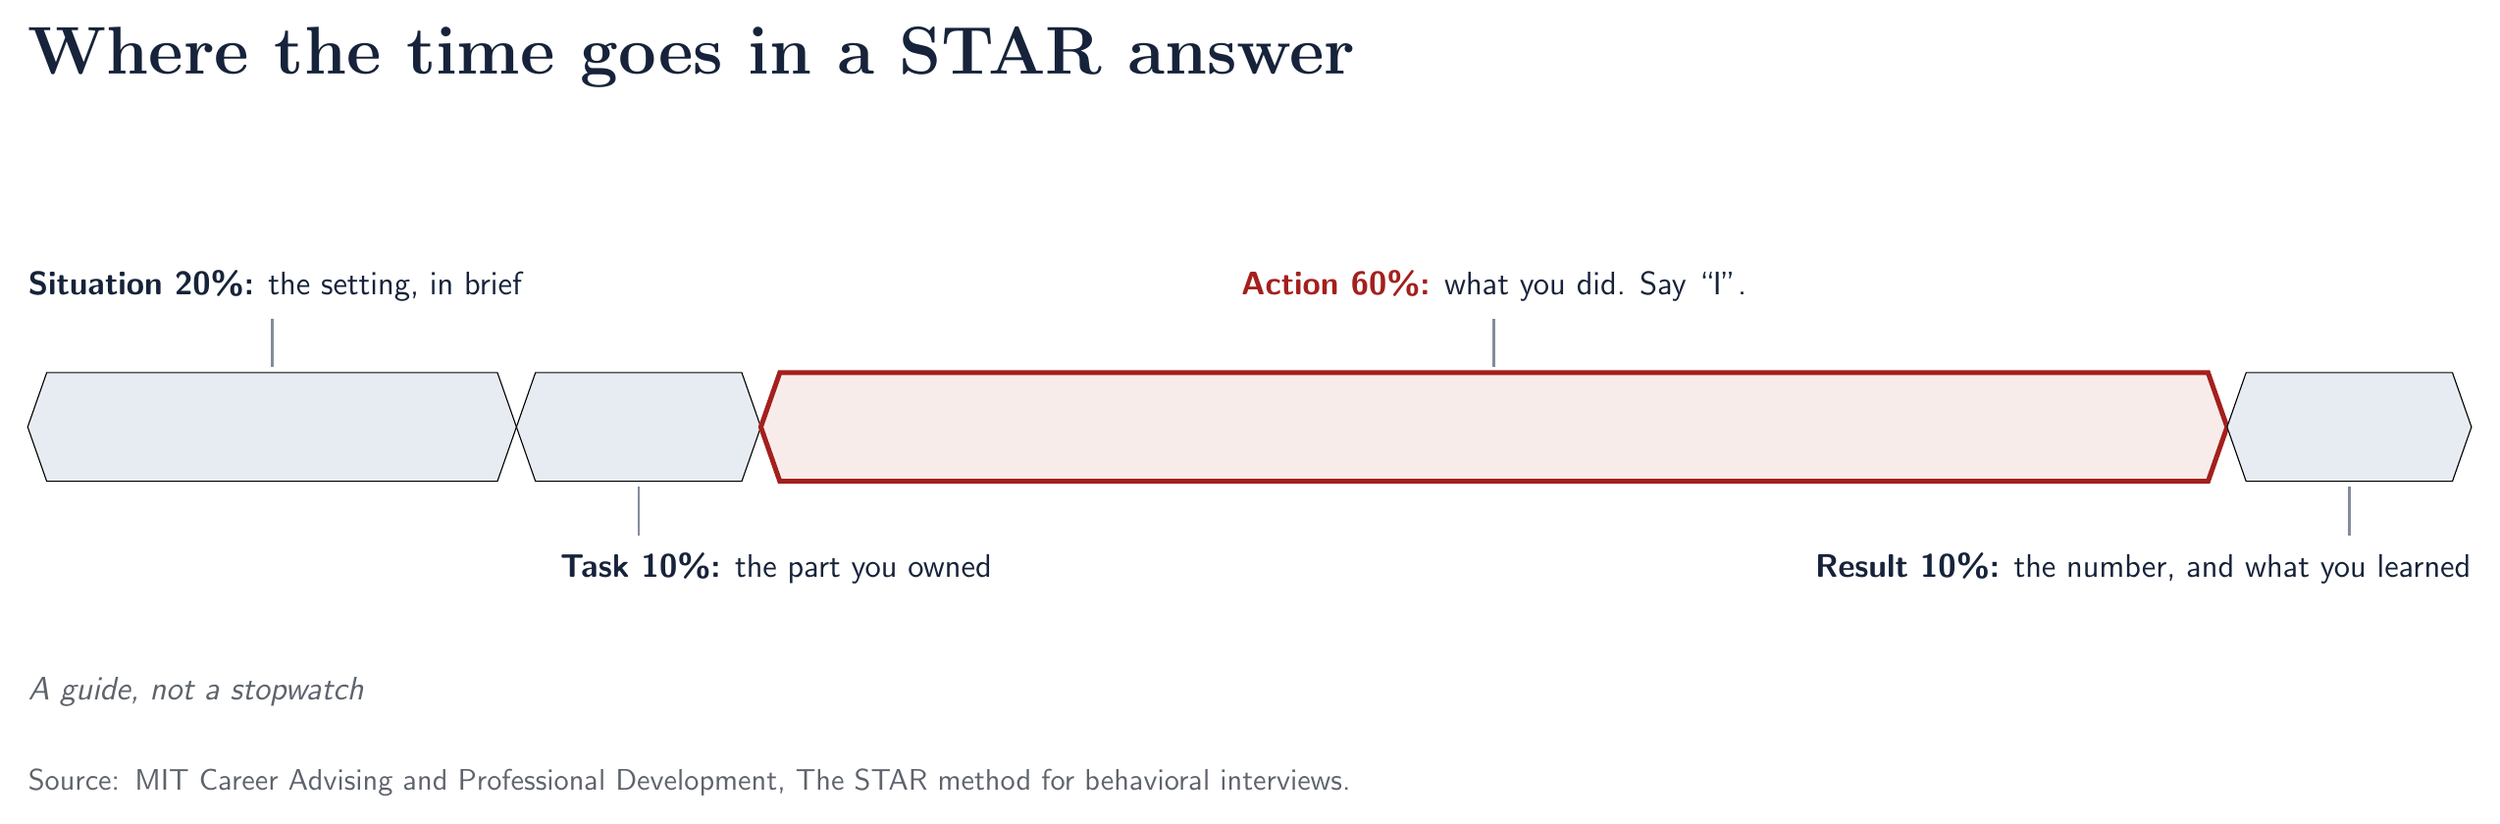
\begin{tikzpicture}[x=1pt,y=-1pt]
  \node[eeptitle] at (0,30) {Where the time goes in a STAR answer};
  \seg{0}{180}{fill=eepwash}
  \seg{180}{270}{fill=eepwash}
  \seg{270}{810}{draw=eepaccent, line width=1.8pt, fill=eepaccentsoft}
  \seg{810}{900}{fill=eepwash}
  % Leaders and labels: two above, two below.
  \draw[eeplead] (90,138) -- (90,120);  \draw[eeplead] (540,138) -- (540,120);
  \draw[eeplead] (225,182) -- (225,200); \draw[eeplead] (855,182) -- (855,200);
  \node[eepbody, text=eepink, anchor=south west] at (0,114) {\textbf{Situation 20\%:} the setting, in brief};
  \node[eepbody, text=eepink, anchor=south] at (540,114) {\textcolor{eepaccent}{\textbf{Action 60\%:}} what you did. Say “I”.};
  \node[eepbody, text=eepink, anchor=north west] at (196,206) {\textbf{Task 10\%:} the part you owned};
  \node[eepbody, text=eepink, anchor=north east] at (900,206) {\textbf{Result 10\%:} the number, and what you learned};
  \node[eepnote, anchor=north west, font=\sffamily\itshape\fontsize{12.5}{16}\selectfont] at (0,252) {A guide, not a stopwatch};
  \node[eepsrc, text width=900pt] at (0,286) {Source: MIT Career Advising and Professional Development, The STAR method for behavioral interviews.};
\end{tikzpicture}
\end{document}
